The goal of NEAT is to make topological units modular.  
These can then be combined in a not predetermined way.  
So our two questions while combining become:  
\begin{enumerate}
	\item{How can we make CNN's modular?}  
	\item{How can combine these units in a meaningful way?}  
\end{enumerate}

Our first approach was simply taking NEAT and exchanging some of the neurons for Filters.  
An example network can be seen here:  

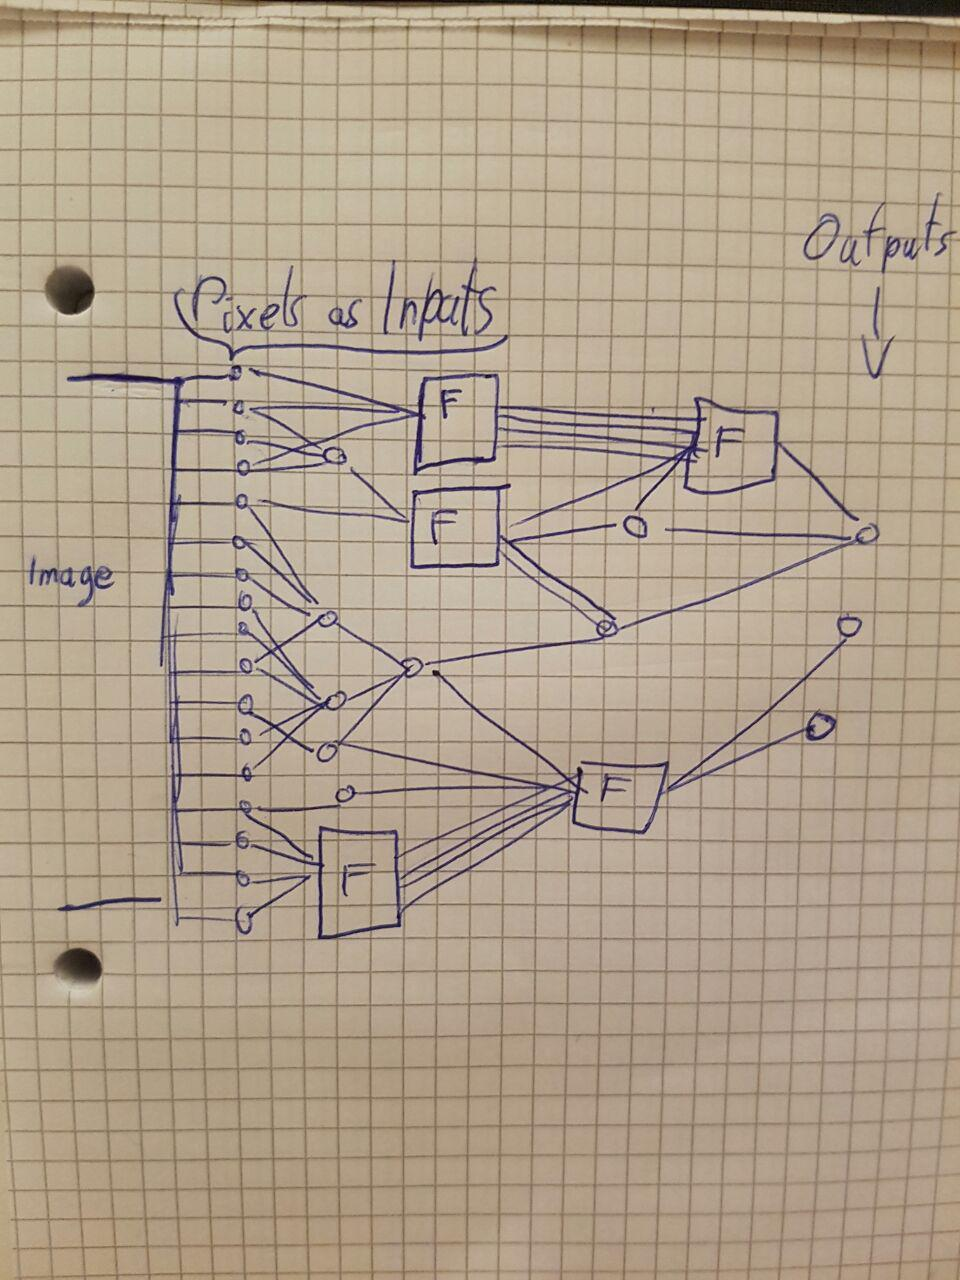
\includegraphics[scale=0.4]{approachone.jpg}  

This approach is probably as modular as it gets, however it brings various problems when combining.  
\begin{enumerate}
	\item{We ignore one of the main advantages on CNN: Being able to drastically lower the number of inputs through subsampling}
	\item{We don't use Pooling or ReLU layers}
	\item{The significance of a single classic neuron in such a system is questionable}
	\item{The filters in the same layer have to have some way of communicating to form a convolution}
	\item{Adding a new filter in a convolution conflicts with previous learned parameters}
\end{enumerate}

We can't address all of these conflicts in a satisfactory way, so we decided to go on to a next approach.
\\
We adressed issue 3 by separating the whole network into a convolutional and a fully connected part. This allows us to takle issue 1 by adding the concept of a \emph{minimal network}, inspired by NEAT's practice of always starting by combining all inputs with all outputs.  
In our case, the minimal network would incorporate some combination of convolution and pooling to reduce the input space. While the exact form of it is debatable, we think a good starting point is LeNet, as it proved itself to be flexible in it's application. \cite{YannLeCun1998}  
\\
The overhauled version would start out like this:  
\\
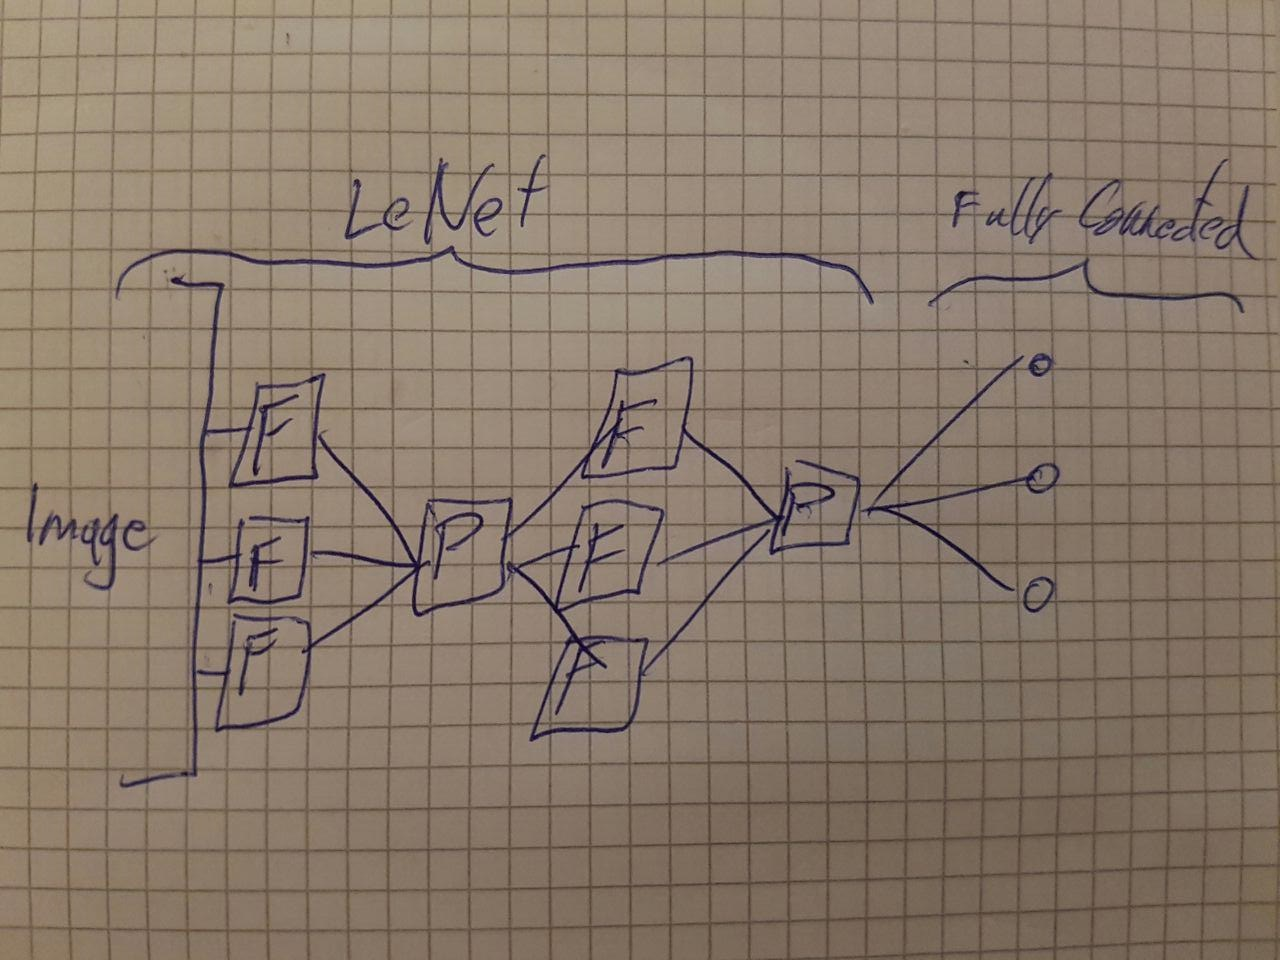
\includegraphics[scale=0.4]{approachtwoinit.jpg}  
\\
And could evolve into something like this:
\\
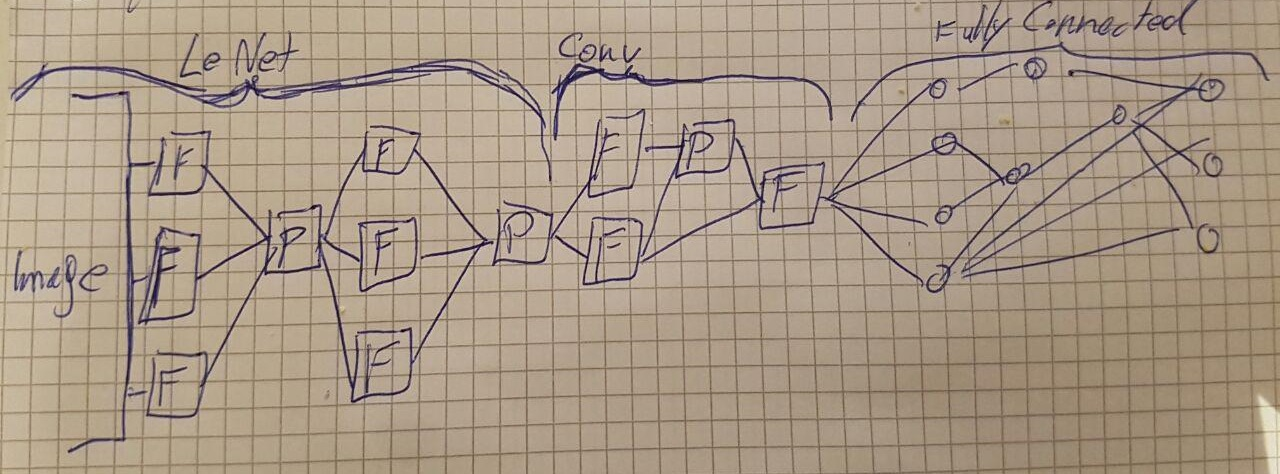
\includegraphics[scale=0.4]{approachtwoevolved.jpg}  
\\

This raises a new question: \emph{How is the meaning of the fully connected part altered when we add a new unit in the convolutional part?}  
After detailed evaluation, we came to the conclusion that the parameters of the fully connected part would be fine tuned to a specific expected input. This expectation however ceases to be met once the dimensionality of the convolutions changes, as this shifts a lot of weight parameters towards a new meaning.  
This means that we have two choices in case of a topological change in the convolutional part:
\begin{enumerate}
	\item{Adjust weights for the new meaning}
	\item{Trash the fully connected part and train it anew}
\end{enumerate}  
Both of these possibilities are not satisfactory. 1 will take a long time, since the already trained structure is basically meaningless now. 2 throws away big, otherwise perfectly usable, parts of the network.  

